\section{Communication}
Dans le but de faire communiquer les voitures et les feux, nous avons mis en place 3 outils de communication. Une file de message a été nécessaire pour stocker les requetes des bus arrivant dans une voie. Cette file contient des structures de type requeteBus. Nous avons également eu besoin d'une mémoire partagée. Elle contient l'état actuel des feux grâce à une structure de type feu. Enfin, une dernière mémoire partagée nous a servi à contrôler le nombre de voitures arrivant dans chaque voie de sortie.
\newpage
\begin{figure}[htb!]
\centering
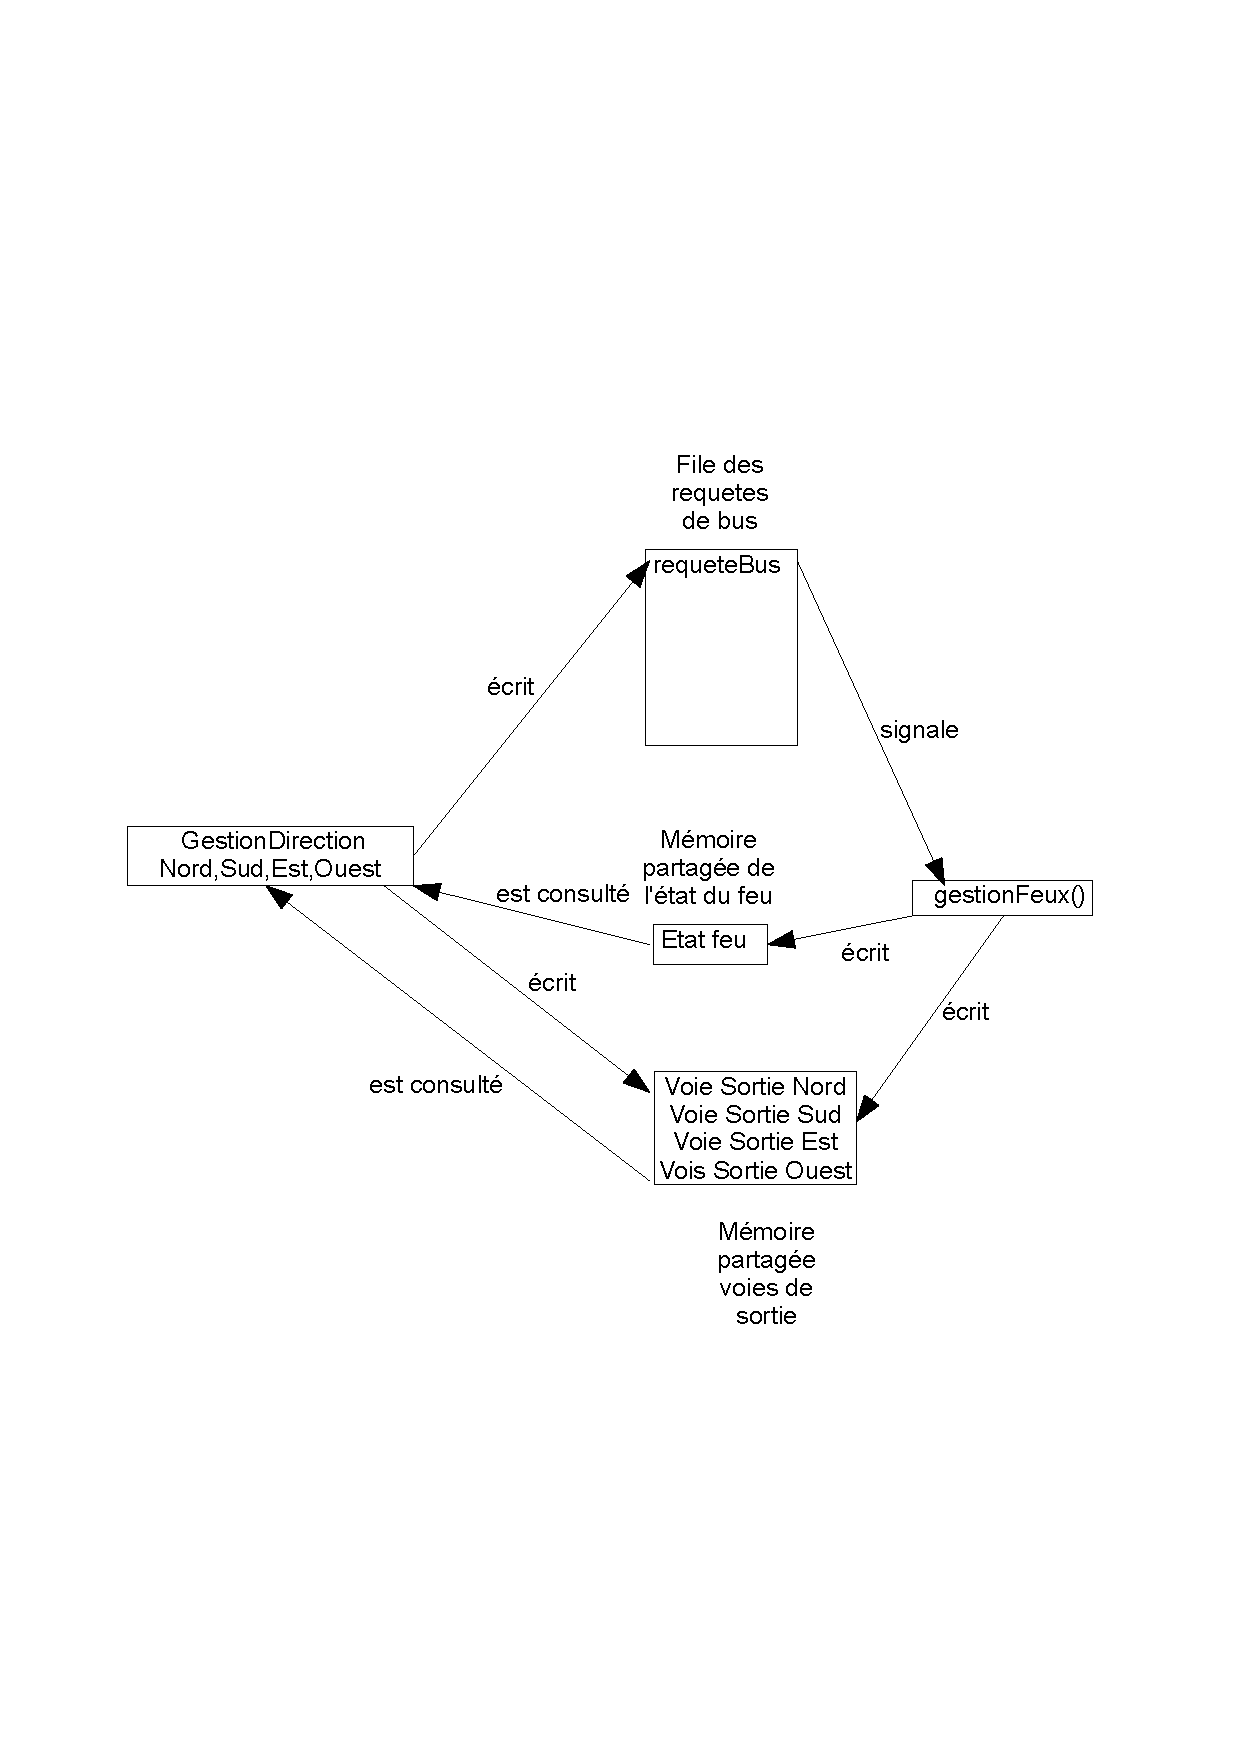
\includegraphics[scale=0.5]{graphe1LO41.pdf}

\caption{Accès des processus aux mémoires}
\end{figure}
